 \asection{Search Matching Algorithm}
\label{Search Matching Algorithm}


\subsection{Introduction}
Subgraph ismorphis can be determined using a brute-force approach on the tree representation of a graph $G${\tiny A}. Though this technique is effective, it is however not efficient, this is because all the possible permutation subgraphs of a graph $G${\tiny A} are tested against the graph $G${\tiny B} to determine if there are subgraphs in graph $G${\tiny A} that are isomorphic to graph $G${\tiny B}.The number of subgraphs of a graph $G${\tiny A} increase at an exponential rate with every addition of a vertice $V${\tiny n} into the graph, thus the total number of subgraphs that can be evaluated are  
	\begin{equation}
		ST = 2^{n/2}
	\end{equation} where $ST$ is the total number of subgraphs and $n$ the number if vertices in the graph $G${\tiny A}.\newline\newline
The matching process is computationally expensive due to this very fact, that is the more vertices there are in the graph $G${\tiny A}, the more expensive it becomes to detect the subgraph ismorphisms because of the amount of subgraphs it has and thus must be evaluated.\newline\newline This paper explores two graphs that are very effective with regards to graph isomorphis and sub-graph isomorphism detection. The algorithms that are invesicated are the Ullman Algorithm and the VF2 algorithm. \newpage

\subsection{Ullman Algorithm}
\label{Ullman Algorithm}

\subsubsection{Algorithm}
The Ullman algorithm was developed by J.R.Ullman and was published in his paper titled "An Algorithm for Subgraph Isomorphism" [1].The algorithm performs graph matching on an adjacency matrix representation of both the graphs, and uses the depth search first(DSF) recursicve approach to traverse through the graphs and perform the graph matching process. The Ullman algorithm improves the effiency of the brute-force approach at detecting subgraph ismorphisms by deductively eleminating nodes in the tree that are in graph $G${\tiny A}, but are not in graph $G${\tiny B}, thus reducing the number of subgraphs that are matched against graph $G${\tiny B} to determine ismorphism.\newline\newline The algorithm starts by building a starting adjacency matrix $M0$ using the two adjacency matrix representations of graphs $G${\tiny A} and $G${\tiny B} using the following procedure.
\begin{myEnumerate}
\item Construct a $n * m$ matrix where $n$ is the number of rows of graph $G${\tiny B} and $m$ is the number of colums of graph $G${\tiny A}.
\item Set all the entries in the matrix to the value of 1.
\item Apply the following rule:
	Set the values in $M0$ to 0 for all $M0${\tiny ij} where the degree of a vertice in graph $G${\tiny A} at $j$ is greater then the degree of the same vertice in graph $G${\tiny B} .i.e. 
	\begin{equation}
		deg(Ai) < deg(Bj). 
	\end{equation}

\end{myEnumerate}
	A more formal representation of this rule is as follows
	\[
			f(x)= 
			\begin{cases}
				1,& \text{if } deg(Ai)\geq deg(Bj)\\ 
				0,              & \text{otherwise}\   \forall \text{i,j}
			\end{cases}
	\]
When the starting matrix has been constructed, we systematically permute matrices $M^d$ from the starting matrix $M0$ where $d$ represents the depth of the generated matrix. The procedure of generating the permuted matrices follows a depth search first (DSF) recursicve approach where the stopping condition (leaf matrices) conform to the following form:
\begin{myEnumerate}
\item $M$ contains only $0's$ and $1's$.
\item There is exactly one $1$ in each row.
\item Not more than one $1$ in each colum.
\end{myEnumerate}
An demonstration of how the permutation matrices are generated is demonstrated in figure ~\ref{fig:permutationmatrix}.

\begin{figure}[H]
  \begin{center}
      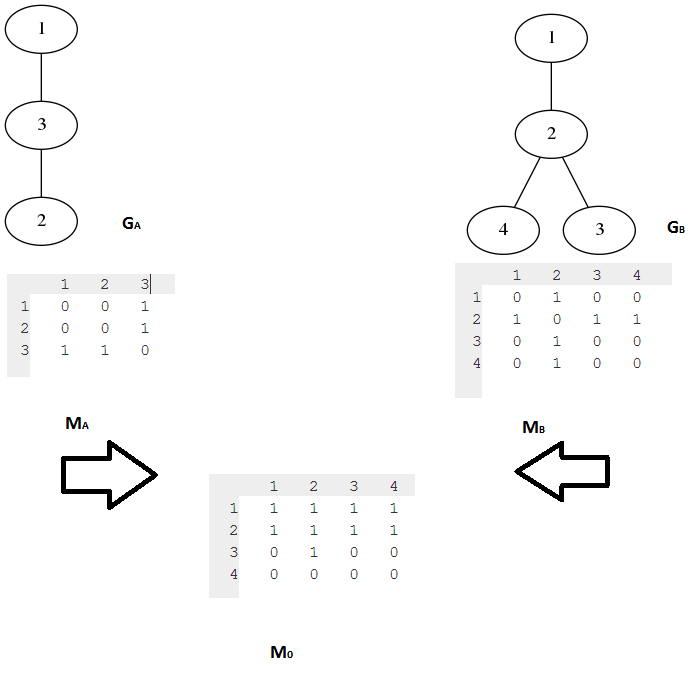
\includegraphics[width=0.65\textwidth]{stratMatrix}
  \end{center}    
  \caption{Demonstation of how a permutation matrix is generated from two graphs} 
  \label{fig:permutationmatrix}
\end{figure} 
Once all the permutation matrices have been generated, each one of the matrices is matched with a graph $C$, that is obtained from the dot product of the permuted matrix and the graph $G${\tiny A}.
The formula for calculating graph $C$ is follows:
$C$=$M${\tiny n}($M${\tiny n} . G{\tiny A})T, where $G${\tiny A} = input graph and  $M${\tiny n} = permutated matrix $M${\tiny n} in $M^d$, obtained from the starting matrix $M0$ ($M${\tiny n} . $G${\tiny A})$T$ = the transpose of the dot product of the permutated matrix $M${\tiny n} and the graph $G${\tiny A}.
If there is a single instance of the matrix $C$, that is calculated using some permutated matrix $M${\tiny n} obtained from the starting matrix $M0$, that is equal to matrix $G${\tiny B}, then $G${\tiny B} is isomorphic to $G${\tiny A}. Thus $G${\tiny B} is isomorphic to $G${\tiny A} $iff G${\tiny B}
  \begin{equation}	
	ij = 1 \rightarrow  Cij = 1 \forall i,j
  \end{equation} 
If non of the generated permutated matrices can statisfy this condition, then $G${\tiny B} is not isomorphic to $G${\tiny B}.

\subsubsection{Ullman Pseudo code}
	\begin{figure}[H]
	  \begin{center}
		  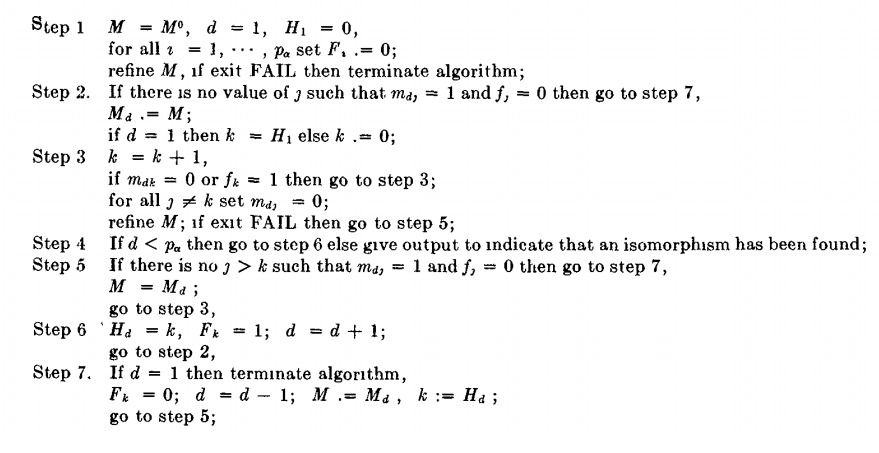
\includegraphics[width=1.0\textwidth]{Ullmanpseudo}
	  \end{center}    
	  \caption{Pseudo code of the Ullman algorith [1]}
	  \label{fig:ullmanpseudo}
	\end{figure} 
\newpage

 \subsection{VF2 Algorithm}
\label{VF2 Algorithm}

\subsubsection{Algorithm}

 The VF2 algorithm was introduced by L.P.Cordella, P.Foggiaa, C.Sansone and M.Vento [11]. The algorithm is suitable for graph matching and isomorphic determination, including subgraph isomorphic determination on large graphs, this is attributed to the Data structures that the algorithm uses and the manner in which they are used [11], this feature is discussed later in the paper.\newline\newline The algorithm performs the matching process by attempting to find a mapping $M$, of vertices in graph $G${\tiny A} which correspond to vertices in graph $G${\tiny B}. The mapping is then used to determine if the two graphs are completely syntactically similar(isomorphic), partially syntactically similar or have no structural similarities at all.

\myparagraph{Matching and Mapping definition}
A mapping $M$ is defined as a set of pairs $(n,m)$, where $n$ is a vertice from $G${\tiny A} and $m$ a vertice from $G${\tiny B}, thus $n \subseteq G${\tiny A} and $m \subseteq G${\tiny B}.\newline\newline
The isomorphism determining properties of the mapping are defined as follows, a mapping $M \subset N${\tiny A} $ * N${\tiny B} is isomorphic $iff M$ is a bijection, that preserves the branching structure of $G${\tiny A} and $G${\tiny B}, where $N${\tiny A} is a set of vertices from $G${\tiny A} and $N${\tiny B} a set of vertices from $G${\tiny B}.\newline\newline
The mapping $M \subset N${\tiny A}$ * N${\tiny B} is subgraph isomorphic $iff M$ is isomorphic to $G${\tiny A} and a subgraph of $G${\tiny B}.

\myparagraph{Mapping Procedure}
The mapping $M$ comprises of state based partial solution morphisms $M(s)$ for each state $s$.The process of finding the mapping $M$ that is described above uses State Space Representations (SSR) [12].
The partial solution morphisms $M(s)$ selects two subgraphs from $G${\tiny A} and $G${\tiny B}, namely $G${\tiny A}$(s)$ and $G${\tiny B}$(s)$ respectively. The subgraphs comprises of only vertices that are present in the partial solution $M(s)$ for the state $s$ as well as the edges joining them together.\newline\newline
The algorithm starts with an initial state $s0$ that has no mapping between the two graphs, thus $M(s0)= NULL$. The algorithm then computes a set of candidate pairs $P(s)$. Each candidate $p$ in the set is checked against the feasibility function that is discussed in the following chapter, if $p$ is successful then it is added to the state $s$. And the successor $s'$ is computed using a combination of the predecessor state and the candidate $p$, thus:
	\begin{equation}
		s' = s \cup p
	\end{equation}
The process of generating successor states is a recursive procedure that makes use of the depth first traversal for graphs. When a path has been 
exhausted and a solution has not yet been found, the algorithm uses backtracking to explore the alternative paths [11,13]. \newpage

\myparagraph{Definition of the set $P(s)$ and of the feasibility function $F(s, n, m)$}
The VF2 algorithm generates the states with close consideration that only some of the states are consistant with the desired morphisms [12]. The algorithm avoids inconsistant states by making use of a set of rules in it's state generation procedure, thus ensuring that only consistant state are generated, these rules are refered to as feasibility rules.\newline\newline The algorithm uses a function called a feasibility function to test that an additon of a pair $(n,m)$ to a state will be consistant. If the addtion of the pair passes all the feasibility rules, the algorithm will return a true value, if not, a false value indicating that the procedure results in an inconsistant successor  state $s'$, and thus that state $s'$ will not be explored by the algorithm.\newline\newline A further filter can be applied in the consistent states to rule out those states whose successor states will be inconsistant, this apporoach is employed by adding a additional rules called $k-look-ahead$ rules [12]. They check to see if the current state $s$ will have a consistant successor state after $k$ steps, i.e. they check to see if the states from $s$ to $s^k$ are consistant with the desired morphisms.

 \myparagraph{Condidate Pairs}
 The candidate pairs are obtained by considering the vertices that are connect to $G${\tiny A}$(s)$ and $G${\tiny B}$(s)$, the sub-graphs of $G${\tiny A} and $G${\tiny B} in the state $s$. The vertexs are used to form the pairs $(n,m)$ as defined above. In order explain how the pairs are formed, we must first introduce the following definitions:\newline
Let:
\begin{myEnumerate}
\item $T${\tiny A}$in(s)$ be the set of vertexs that are not yet in the partial mapping $M(s)$ and are the origin \quad of the edges from graph $G${\tiny A}
\item $T${\tiny B}$in(s)$ be the set of vertexs that are not yet in the partial mapping $M(s)$ and are the origin of the edges from graph $G${\tiny B}
\item $T${\tiny A}$out(s)$ be the set of vertexs that are not yet in the partial mapping $M(s)$ and are the destination of the edges from graph $G${\tiny A}
\item $T${\tiny B}$out(s)$ be the set of vertexs that are not yet in the partial mapping $M(s)$ and are the destination of the edges from graph $G${\tiny B}
\end{myEnumerate}

The pair $(n,m)$ is made by vertex $n$ from $T${\tiny A}$out(s)$ and $m$ from $T${\tiny B}$out(s)$. If the any of the sets is empty, then we consider the vertex $n$ from $T${\tiny A}$in(s)$ and $m$ from $T${\tiny B}$in(s)$. In the case where that graphs are not connected, the pairs will be made by all the vertex not yet contained in either $G${\tiny A}$(s)$ and $G${\tiny B}$(s)$. These pairs form the entries in the set $P(s)$ for that respective state $s$.

\myparagraph{The feasibility rules}
The feasibility rules that are used to ensure that the states that are evaluated play a role in improving the performance, by preventing inconsistent states from being explored and thus optimizing the execution of the algorithm. There are five general feasibility rules defined as $R${\tiny pred},$R${\tiny succ},$R${\tiny in},$R${\tiny out} and $R${\tiny new} respectively.\newline\newline The feasibility functions check for two main things, firstly they check the consistency of the partial solution in the successor state $s'$, namely $M(s')$. Rules $R${\tiny pred} and $R${\tiny succ} are the rules used for this checking.\newline
The remaining rules are used for pruning the search space for different levels of look ahead. The $R${\tiny in} and $R${\tiny out} are used to look ahead one level and determine which of those successor states are consistent, and $R${\tiny new} is used for the same purpose, but for a look ahead level of two. The definition for each rule is as follows:


\subimport{}{rules}
\newpage
In order for a state to be considered consistent, it must pass a combination of all of the five rules, namely:
	\begin{equation}
		Fsyn(s,n,m) = Rpred \wedge Rsucc \wedge Rin \wedge Rout \wedge Rnew 
	\end{equation} 

where $F${\tiny syn}$(s,n,m)$ the feasibility function that is envoked upon the state $s$.

\subsubsection{VF2 Pseudo code}
	\begin{figure}[H]
	  \begin{center}
		  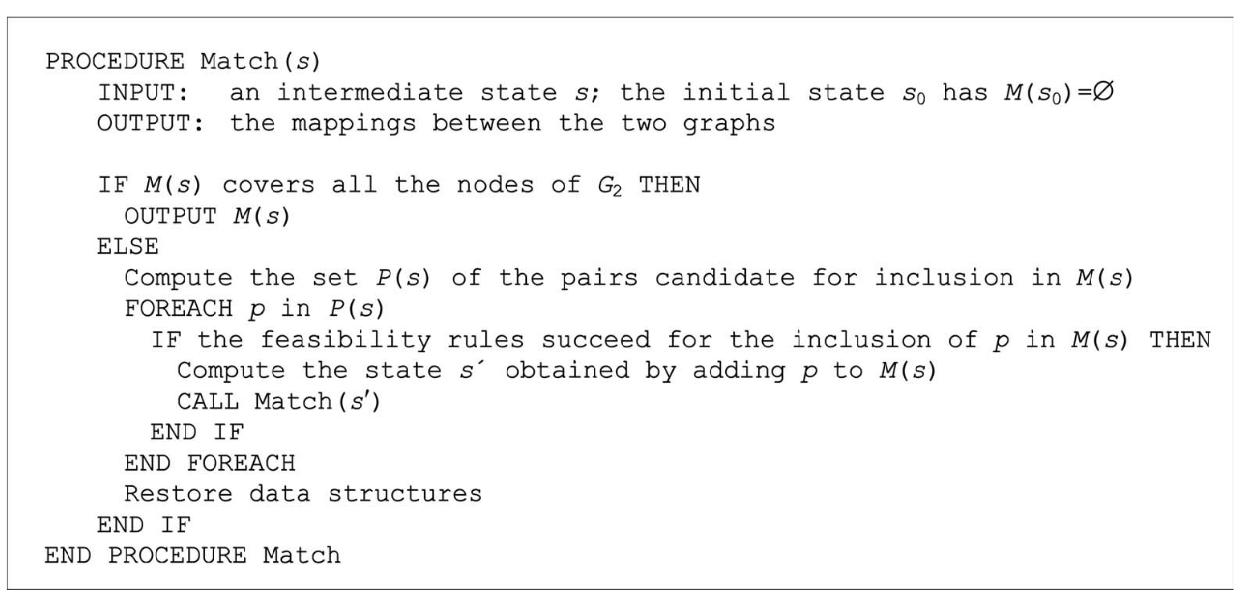
\includegraphics[width=1.0\textwidth]{VF2pseudo}
	  \end{center}    
	  \caption{Pseudo code of the VF2 algorith [11]}
	  \label{fig:vf2pseudo}
	\end{figure} 

 \subsection{Conclusion}

 The Ullman and VF2 algorithm that are discussed above both follow a similar approach in attempting to perform graph mathing. They both construct a tree from the adjacency representation of their input graphs and use the depth first tree traversal techniques to evaluate the graphs, this is done every effectively by both the algorithms.\newline\newline
 Though both algorithms are effective in their own respective regards, they are optimized rather differently and thus differe in their degree of complexity. The VF2 algorithm optimizes its execution by performing a look-ahead operation of two states from its current states in an attempt to ignore paths that will result in inconsistant states.\newline\newline
 The Ullman algorithm on the other hand optimizes its execution by not computing all possible sub-graphs of some graph $G$, but reduces the computated matrices by initially computing a matrice $M0$ from the input graphs and then ensuring that all the matrices that are computed from $M0$ are tested so as to prevent the algorithm from exploring a branch that will not result in a graph or sub-graph isomorphism
\newpage

